\documentclass[12pt,a4paper]{article}
%\usepackage[onehalfspacing]{setspace}
\usepackage{minted}
\usepackage{url}
\usepackage{graphicx}
\bibliographystyle{ieeepes}
\title{Multiplication of Two BigNums on a Nvidia Graphic Card}
\author{Johannes H\"abe  \\
	jh-191149@hs-weingarten.de
	\and 
	Maximilian Nestle \\
	mn-192181@hs-weingarten.de \\\\
	Ravensburg-Weingarten University of Applied Sciences
	}

\date{\today}
% Hint: \title{what ever}, \author{who care} and \date{when ever} could stand 
% before or after the \begin{document} command 
% BUT the \maketitle command MUST come AFTER the \begin{document} command! 
\begin{document}
\maketitle
%
\begin{abstract}
This paper is about testing the performance of the NVIDIA CUDA Fast Fourier Transform library (cuFFT) by multiplying two large numbers (BigNums) on the graphics card. The performance is measured up to the size of 28.000 bits for each factor. These two factors were also multiplied on the CPU using the Karatsuba algorithm and compared to the cuFFT results. It turned out that the performance on the CPU is one hundred times faster than the multiplication on the GPU comparing a bit range from 24 bit up to 28.000 bits by continuously increasing the size of the factors by 24 Bit. The measured times between the CPU and GPU are resulting in gradually approaching functions.
\end{abstract}

\section{Introduction}
The fast multiplication of two large prime numbers is necessary in some procedures to attack asymmetrical encryption algorithms like the RSA encryption. These computations are normally made on the CPU. Classical approaches have $O(n^2)$ complexity, but polynomial multiplication with FFT has $O(n \cdot logn)$ complexity \cite{bantikyan2014big}. Within this paper, General Purpose Computing On GPUs (GPGPU) is used to multiply BigNums with the help of the NVIDIA CUDA Fast Fourier Transform library (cuFFT). For this purpose, the computing time of BigNum multiplication on CPU and GPU is compared and evaluated in this paper.

\section{Related Work}
Hovhannes Bantikyan from the University of Armenia did time measurements up to the size of 200.000 digits for each factor and compared the results with other BigNum multiplication libraries such as the GNU Multiple Precision Arithmetic Library \cite{bantikyan2014big}. In contrast to that, the results of cuFFT are compared with the \mintinline{c}{BN_mul()} function from the openssl library in this paper. The size of the factors is also increased and measured in smaller steps of 24 bits. Ando Emerencia also included time measurements in his paper "Multiplying huge Integers using Fourier Transforms" \cite{emerencia2007multiplying}. He compared time measurements of mulitplications with different bases, furthermore he did Maximum Square Error tests.

\section{Technical Background}

\subsection{Fast Fourier Transformation}
The Fast Fourier Transformation (FFT) is based on the Discrete Fourier Transformation (DFT). The DFT of a vector $(x_{0},\dots ,x_{{2n-1}})$ of the size $2n$ is \cite{wiki:fft}:
\begin{center}
$$f_m = \sum_{k=0}^{2n-1}x_k \cdot e^{-\frac{2\pi \cdot i}{2n}mk} \quad$$ with $\quad m = 0,\dots,2n-1$.
\end{center}
Fast Fourier Transformation can be used to perform fast integer multiplication via fast polynomial multiplication. CUFFT Library employs the Cooley-Tukey algorithm to reduce the number of required operations resulting in $O(n \cdot logn)$ complexity \cite{nvidia2012cuda}. The resulting complexity is reached by an divide and conquer approach \cite{bekele2016cooley}.
Radix-2 decimation-in-time (DIT), which is the simplest and most common form of the Cooley–Tukey algorithm, first computes the DFTs of the even-indexed inputs and then the odd-indexed inputs. In the end it combines those two results to produce the DFT of the whole sequence \cite{wiki:xxx}. By performing this recursively, the overall runtime can be reduced to $O(n \cdot logn)$.

\subsection{Features GPU and CPU}
CPUs have less cores than GPUs, but the cores are more powerful, visualized in figure \ref{cpu_gpu_cores}. GPUs that are used in modern computers do have hundreds of cores and many more threads, thus they are very effective in parallel computing \cite{Palacios2011ACO}. Parallel Computing speeds up the process when multiplying two numbers, because multiplication is always a process of many tiny multiplications that are summed up. Computations on the CPU are preferred when multiplying tiny numbers, because of the low memory access times \cite{albers2009grafik}.

\begin{figure}[hbt!]
\centering 
\caption{CPU cores (blue) and GPU cores (green)}
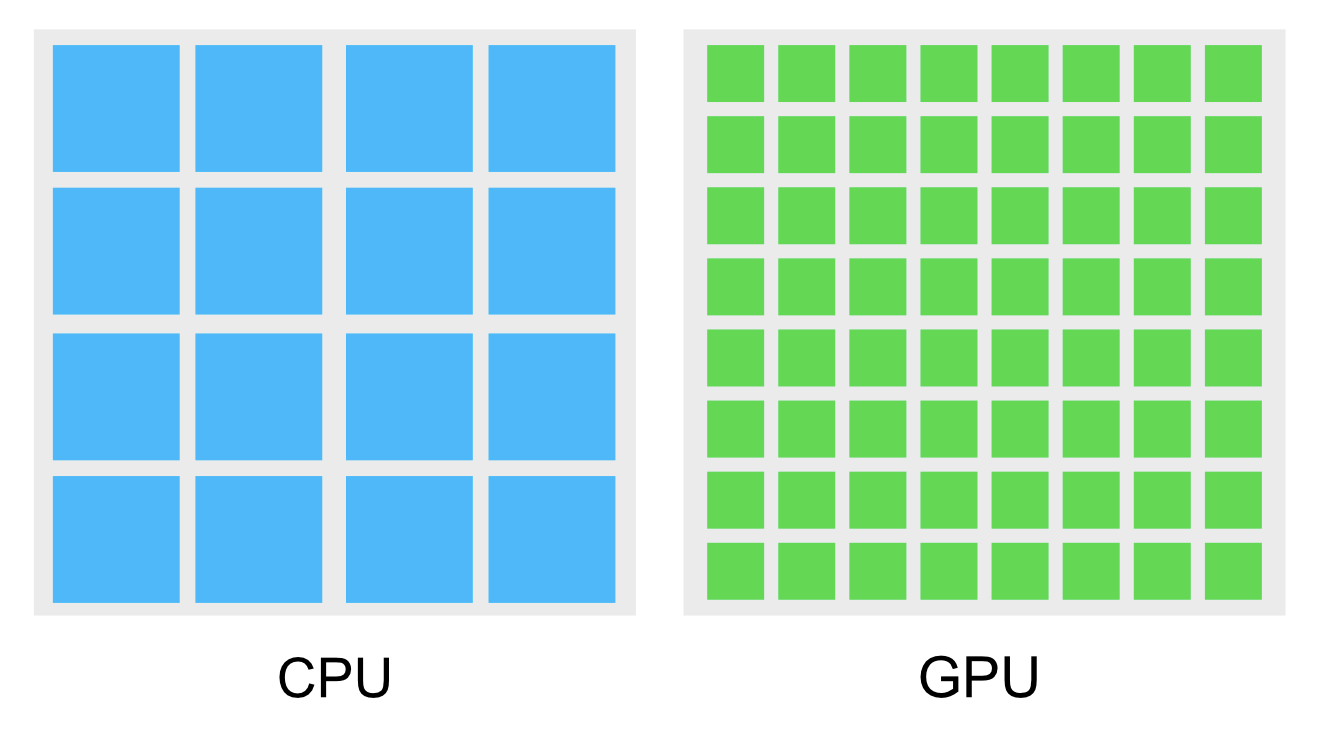
\includegraphics[scale=0.33]{cpugpu.png}
\label{cpu_gpu_cores} 
\end{figure}

\section{Methodology}
For the multiplications an Acer Aspire V3-772G is used. The Acer has got a NVIDIA GTX 850M graphics card and an Intel Core i5 4200M CPU. The graphics card disposes of 2004 MIB storage. The Acer is running the Linux distribution Ubuntu. The code that is used to multiply two BigNums on the GPU is using the cuFFT library from NVIDIA. The multiplications on the CPU are done with the \mintinline{c}{BN_mul()} function from the openssl library which is based on the Karatsuba algorithm \cite{young1995bnmul}, having $O(n^{1.585})$ complexity \cite{dietzfelbinger2012eff}. Two different algorithms are chosen, because most of the BigNum multiplication libraries for the CPU use Karatsuba, but NVIDIA is specialized on cuFFT.

The computation time for the multiplications of the two numbers is measured up to the size of 28.000 bits for each factor. The step size for the multiplications is 24 bits. That means that computations are done for numbers of the size 24 bits, 48 bits, 72 bits and so on. The numbers used for computations are created randomly. To prevent variations caused by random created numbers that are easy to multiply, one hundred multiplications, each with random numbers, are done for each step of 24 bits.

\section{Results}
For the time measurement the C library function \mintinline{c}{clock()} is used. The legend of the measured times is explained in table \ref{Description}. In table \ref{AvgMaxMin} the minimum, maximum and average times for the calculations from 24 bits to 28800 bits are listed. The minimum for all seven categories is located between 24 and 120 bits, the maximum was always close to 28.000 bits. Table \ref{AvgMaxMin} shows, that GPU\_Alloc and CUDA\_Pre cost by far most of the time. They are each in average more than a hundred times slower than the CPU.

\begin{table}
\centering
\caption{Descriptions of the abbreviations of the measured times.}
\vspace{0.5cm}
\label{Description}
\begin{tabular}{p{2cm}|p{9.0cm}|}
\cline{1-2}
 \multicolumn{1}{|l|}{CPU} & The time needed for the multiplications of the two BigNums on the CPU using the \mintinline{c}{BN_mul()} function. \\ \hline
 \multicolumn{1}{|l|}{GPU\_All} & The sum of the times needed for GPU\_Alloc, GPU\_Calc, GPU\_Clean, CUDA\_Pre, and CUDA\_Post. \\ \hline
 \multicolumn{1}{|l|}{GPU\_Alloc} & The time needed to allocate the amount of graphics card memory needed for the two BigNums using \mintinline{c}{cudaMalloc()} and copying them to the graphics card memory by using \mintinline{c}{cudaMemcpy()}.
 \\ \hline
 \multicolumn{1}{|l|}{GPU\_Calc} & The amount of time needed for the calculation of the two BigNums on the GPU. This includes converting the BigNums to frequency domain, multiplying them with \mintinline{c}{ComplexPointwiseMulAndScale()} and converting them back to time domain. \\ \hline
 \multicolumn{1}{|l|}{GPU\_Clean} & The sum of the times needed to copy the data back to the host by using \mintinline{c}{cudaMemcpy()} and to free the graphics card memory by using \mintinline{c}{cufftDestroy()} and \mintinline{c}{cudaFree()}.\\ \hline
 \multicolumn{1}{|l|}{CUDA\_Pre} & The time needed to prepare the data for the multiplication. The algorithm needs to convert the two numbers from the datatype BigNum to float vectors. Float vectors are required for the \mintinline{c}{cudaMemcpy()} function. Also the size of the vectors needs to be adjusted, because cuFFT saves the solution in one of the initial BigNums. \\ \hline
 \multicolumn{1}{|l|}{CUDA\_Post} & The time needed to prepare the result. This includes removing excess zeros, processing carry and turning the result from a float vector to a BigNum. \\ \hline
\end{tabular}
\end{table}

\begin{table}
\centering
\caption{Average, minimum and maximum times measured of all bit sizes.}
\vspace{0.5cm}
\label{AvgMaxMin}
\begin{tabular}{p{2cm}|p{3cm}|p{3cm}|p{3cm}|}
\cline{2-4}
 & \multicolumn{3}{l|}{Times in seconds}  \\ \hline 
 \multicolumn{1}{|l|}{} & $Minimum$ & $Maximum$ & $Average$\\ \hline
 \multicolumn{1}{|l|}{CPU} & $1 \times 10^{-6}$ & $9 \times 10^{-5}$ & $4,16 \times 10^{-5}$ \\ \hline
 \multicolumn{1}{|l|}{GPU\_All} & $1,72 \times 10^{-3}$ & $1,48 \times 10^{-2}$ & $7,19 \times 10^{-3}$ \\ \hline
 \multicolumn{1}{|l|}{GPU\_Alloc} & $1,42 \times 10^{-3}$ & $6,13 \times 10^{-3}$ & $3,67 \times 10^{-3}$ \\ \hline
 \multicolumn{1}{|l|}{GPU\_Calc} & $8,7 \times 10^{-5}$ & $4,48 \times 10^{-4}$ & $2,45 \times 10^{-4}$ \\ \hline
 \multicolumn{1}{|l|}{GPU\_Clean} & $1,71 \times 10^{-4}$ & $8,17 \times 10^{-4}$ & $4,23 \times 10^{-4}$ \\ \hline
 \multicolumn{1}{|l|}{CUDA\_Pre} & $8 \times 10^{-6}$ & $6,88 \times 10^{-3}$ & $2,44 \times 10^{-3}$ \\ \hline
 \multicolumn{1}{|l|}{CUDA\_Post} & $2 \times 10^{-6}$ & $9,21 \times 10^{-4}$ & $3,97 \times 10^{-4}$ \\ \hline
\end{tabular}
\end{table}

\begin{figure}[hbt!]
\centering 
\caption{GPU\_Calc (blue) and CPU (red) with computed polynomial.}
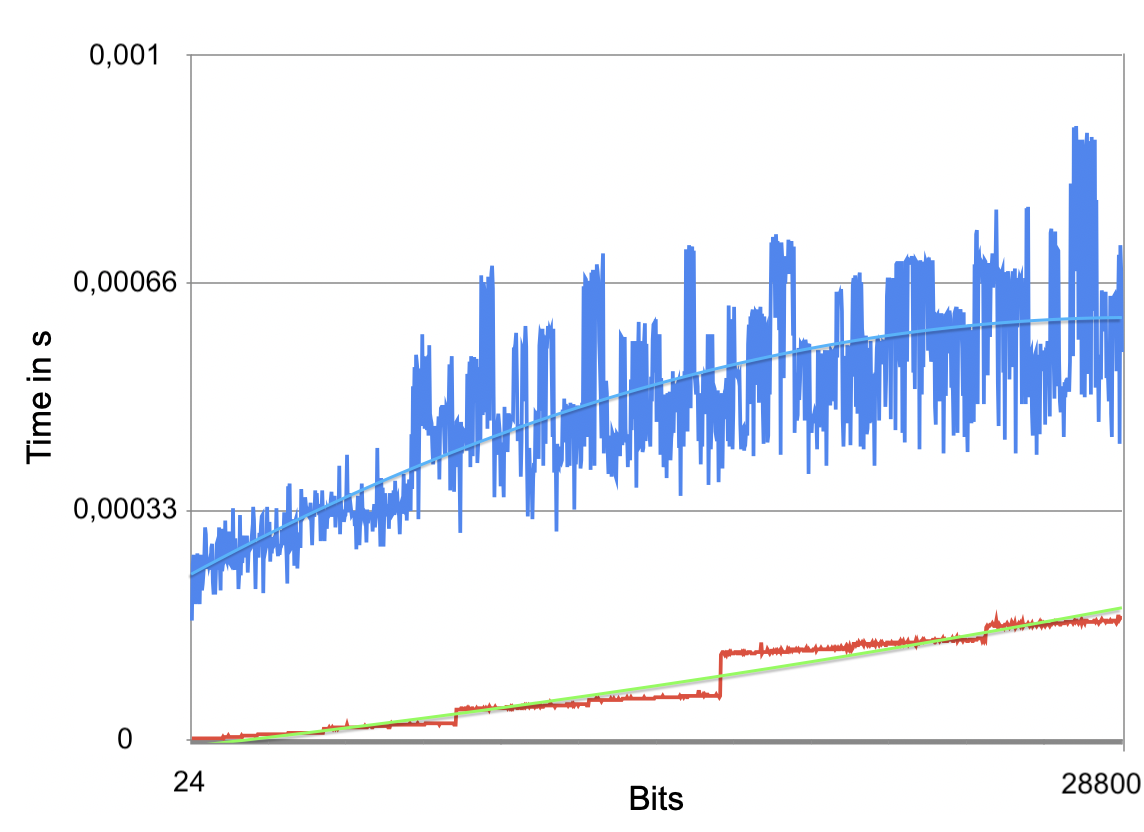
\includegraphics[scale=0.62]{gpucalc_cpu_des.png}
\label{cpugpu_times} 
\end{figure}

The second grade polynomial of GPU\_Calc and CPU were computed and visualized in figure \ref{cpugpu_times} with the original graphs.
 
\begin{center}
    $GPU\_Calc_{poly}(x) = -1.269 \cdot 10^{-10}x^2 + 3.086 \cdot 10^{-7}x + 0.0001$
\end{center}

\begin{center}
    $CPU_{poly}(x) = 1.77 \cdot 10^{-11}x^2 + 6.295 \cdot 10^{-8}x - 4.799 \cdot 10^{-6}$
\end{center}

The slope of the blue polynomial is decreasing, while the slope of the green polynomial is increasing. It can be derived, that the GPU is getting more effective in comparison to the CPU, the bigger the numbers get. This assumption is only valid as long as we use Karatsuba for CPU and FFT for GPU. The graph reflects the complexities of the algorithms.

The measurements were also done on two more computers, to make sure, that the structure of the resulting graphs is nearly the same and not a specific result of the depending hardware of the computers. The assumption was confirmed.

\section{Conclusion}
This paper outlines and indicates that the use of a GPU for BigNum multiplication with factors up to the size of 28.000 bits is not efficient enough. An exception could be multiplying numbers that are heavily bigger than 28.000 bits, because the larger the numbers get, the more effective becomes the multiplication on the GPU. 

The main issues concerning GPUs are the times needed to prepare the data, the allocation of the VRAM and copying data on it. The CPU is able to store all data in cache, while the data transfer on the GPU takes too long \cite{cooper2011gpu}. Even disregarding these time consuming processes of the GPU, it still does not gain much benefit. Then the CPU is up to 28.000 bits still at least 5 times faster than the GPU. The reason for that could be either a worse performance on GPU for numbers up to the size of 28.000 bits, but also could  be caused by the algorithms themselves. Maybe the complexity of FFT compared to Karatsuba only becomes noticeable in much larger numbers.

 With parallel computing of multiple pairs of numbers on the GPU, it can be assumed that the process can be accelerated, for example by allocating a bigger amount of VRAM and putting multiple pairs of numbers on the graphics card memory with just one call of \mintinline{c}{cudaMemcpy()}. Although more performance improvement experiments would be needed to confirm the assertion.

\bibliography{literatur}

\end{document}
